\documentclass[a4paper,12pt]{article}
% \usepackage{mathptmx}
\usepackage{newpxtext,newpxmath} 
\usepackage[notcite,notref]{showkeys} 
\usepackage{graphicx}
\usepackage{tikz}
\usepackage{pgfplots}
% \usepackage{bimatrixgame}
\usetikzlibrary{shapes}
% \usetikzlibrary{arrows}
\usetikzlibrary{arrows.meta}
\pgfplotsset{compat=1.16}
\oddsidemargin=.46cm 
\textwidth=15cm
\textheight=24cm
\topmargin=-1.3cm
\parindent 0pt
\parskip1ex
\pagestyle{empty}
% Line width options: " line width=<dimension> ",
% and abbreviation
% " ultra thin " for 0.1pt,
% " very thin " for 0.2pt,
% " thin " for 0.4pt (the default width),
% " semithick " for 0.6pt,
% " thick " for 0.8pt,
% " very thick " for 1.2pt,
% " ultra thick " for 1.6pt.

% Nim chip
% #1 = height, #2 = horiz offset [scale=.2] 
\newcommand{\chip}[2]{\begin{scope}[shift={(#2,#1)}]
\draw [semithick] (0,0) arc(270:90:0.5) -- (4,1) arc(90:-90:0.5) -- cycle;
\end{scope}}
\newcommand{\HAT}{\hat}
\usepackage{noto}
\newcommand{\prob}{\textup{\small\textsf{prob}}} 
\def\ci#1{{\lower3.4pt\hbox{%
\begin{tikzpicture}[scale=1]
\draw [] (0,0) node[inner sep=1.5pt,thin,draw,circle] {\footnotesize\sf#1};
\end{tikzpicture}}}}
\def\0{{\bf0}} 
\def\T{^{\top}} 
\newsavebox{\figA} 

\begin{document} 

\sbox{\figA}{\ci2}


\hrule
\vskip 2ex

\def\l#1{\footnotesize{\textbf{#1}}}%label
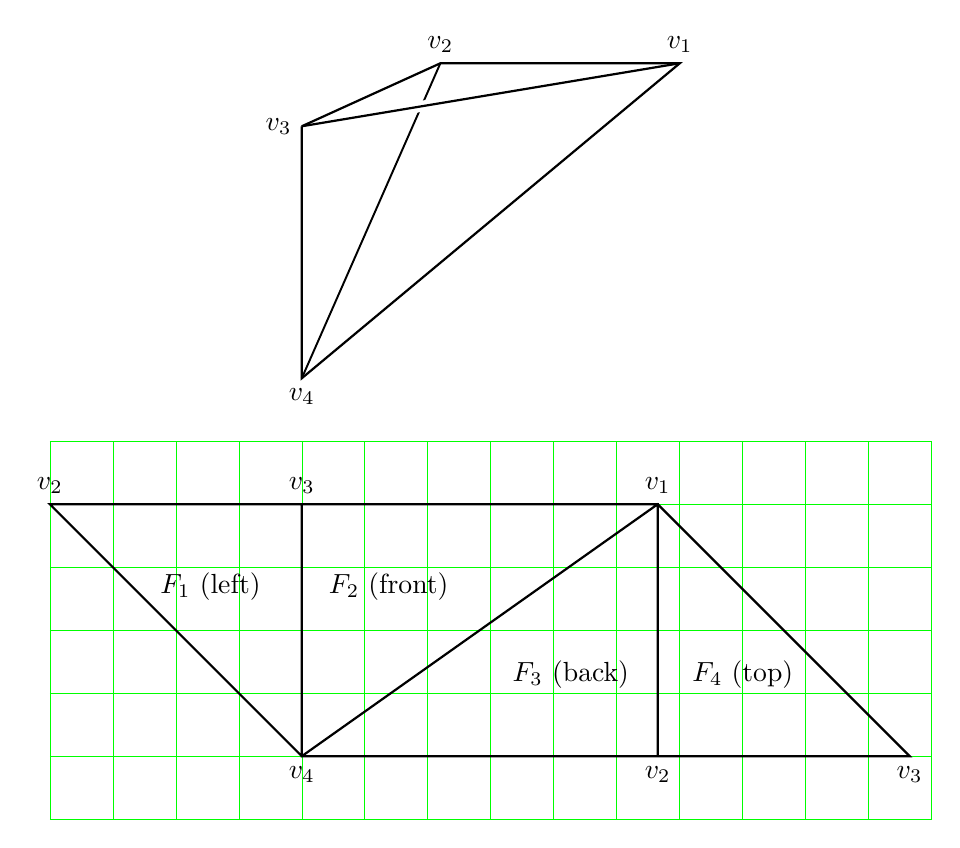
\begin{tikzpicture}[scale=0.8]
\draw [help lines,color=green]  (-4,-1) grid (10,5); 
%\draw (-1,1) node {(a)};
%%%%%%%%%
\begin{scope}[shift={(0,0)}]
\draw [thick] (0,4) node [above] {$v_3$}
  -- (0,0) node [below] {$v_4$}
  -- (9.65,0) node [below] {$v_3$}
  -- (5.65,4) node [above] {$v_1$}
  -- (0,0) 
  -- (-4,4)  node [above] {$v_2$}
  -- (5.65,4) 
  -- (5.65,0) node [below] {$v_2$};
\draw (-1.45,2.7) node {$F_1$ (left)};
\draw (1.38,2.7) node {$F_2$ (front)};
\draw (4.27,1.3) node {$F_3$ (back)};
\draw (7.0,1.3) node {$F_4$ (top)};
\end{scope}
%%%%%%%%%
\begin{scope}[shift={(0,6)}]
% \draw [help lines,color=green]  (-4,-1) grid (10,5); 
\draw [thick] (0,4) node [left] {$v_3$}
  -- (0,0) node [below] {$v_4$}
  -- (6.,5) node [above] {$v_1$}
  -- (2.2,5) node [above] {$v_2$}
  -- (0,4);
\draw [line width = 0.7pt] (0,0) -- (2.2,5) ;
\draw [white,line width = 4pt] (1.8,4.3) -- (2.4,4.4) ;
\draw [thick] (0,4) -- (6.,5) ;
\end{scope}


% \begin{scope}[shift={(-1.75,3.05)}]
% \draw [->] (0.16,0.) arc(0:300:0.16);
% \draw [] (0.,0.) node {$+$\strut};
% \end{scope} 
% \draw [fill] (0,0) circle [radius=0.05];
%%%%%%%%%%%%%%
\end{tikzpicture}
\vskip 2ex
\hrule

\end{document}
